\chapter{Implementation}
\section{Methodology}

\begin{figure}[h]\centering
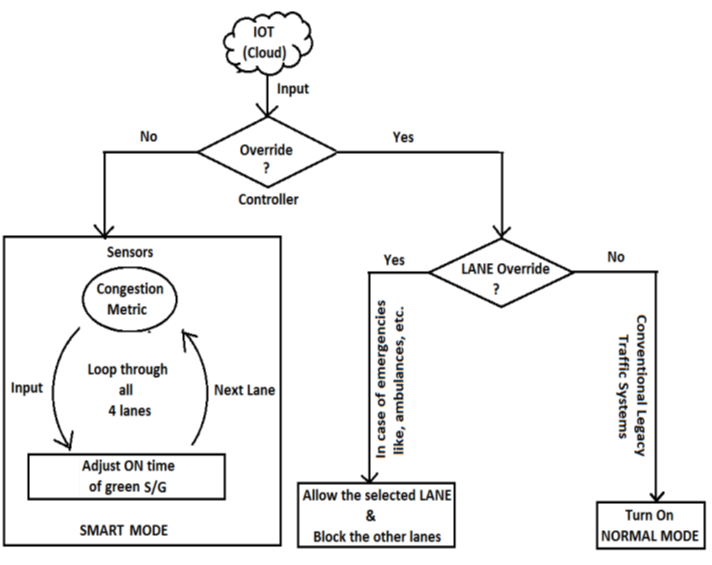
\includegraphics[width=5.5in]{./images/SystemDesign.png}
\caption{Block Diagram of Smart Traffic Control system using IOT}\label{SystemDesign}
\end{figure}
The proposed system mainly operates in two modes,
\begin{itemize}
    \item SMART mode
    \item NORMAL mode
\end{itemize}

\pagebreak

\subsection{SMART MODE}
In SMART mode, the system measures the traffic congestion of a particular lane, by using ultrasonic sensors, in REAL-TIME. The traffic congestion is measured in terms of the distance till which the vehicles are stacked in that lane, which is in direct correlation with the traffic present in that respective lane. The distance is measured using the US sensor with the help of equation 3.1, which can be further simplified down as,

Distance = ((echo pulse period × velocity of sound (330m/s))/2 (4.1)

Here, the distance measured is divided by two since the time for which echo pulse is high is the duration from transmission of ultrasonic signal to it being received back by the sensor after reflecting back from the obstacle. Since, it includes both to and fro motion, the calculated distance is twice that of the distance between sensor and the obstacle. Thus, the measured distance is divided by 2 to get the actual distance.

Once the distance, that gives the measure of congestion of a lane is calculated, the amount of time for which that particular lane vehicles are to be allowed is estimated using an internal algorithm.

\vspace{1cm}

\textbf{Green Time Estimation Algorithm Using Distance}

The basic idea of the algorithm is to estimate time for which the green signal is to be turned on such that, the lane along which there is large congestion/traffic must be allowed for a long time when compared to that of the lane in which the traffic is less. This process ensures that the congestion of the circle is distributed in a balanced manner and equity is given for all lanes.

To accomplish this, a threshold distance and a threshold time is selected (that will be used in case of NORMAL mode), which is the ideal time for which the given lane must be turned on provided, that lane has a traffic corresponding to a distance equal to threshold distance. Based on this setup, now the green time is estimated such that some extra time is added to this threshold value when the actual measured distance is greater than the threshold distance and similarly, some extra time is deducted from the threshold time, when the distance measured is less than the threshold distance.

This extra time that is to be added/subtracted from the threshold value is computed such that it is proportional to the difference in the actual distance and the threshold distance. It is calculated as follows, 

Delta Time = Threshold Time × ((Actual distance – Threshold distance))/(Threshold distance) (4.2)

From the above equation, we see that the value of the (Delta time) > 0, when actual distance measured crosses the threshold and it is < 0, when the actual distance is within the threshold. Now, the final estimated time for which the green time should be turned ON for that particular lane is given by,

Estimated GREEN TIME = Threshold Time + Delta Time (4.3)

From the above equation, we see that, the estimated green time is greater than the threshold value, when the actual distance measured is over-shooting the threshold distance (indicating more traffic density) and is less than the threshold value, when the actual traffic is within the threshold distance. Thus, the estimated green time will be calibrated such that it is proportional to the actual congestion that is being measured in real time and there by operates in an adaptive manner to ensure smooth flow of the traffic.

This process is repeated continuously, in a cyclic manner from LANE-1, LANE-2, LANE-3, LANE-4 and back to LANE-1, using the round-robin method.

\pagebreak

\subsection{NORMAL MODE}

In this mode, the model operates like any other conventional traffic system, where the time for which the green signal is to be turned ON is preset. The system cycles through each lane of the signal with this preset timer value. This value is equal to the threshold time that is used in the SMART mode. The system can be toggled back and forth between these two modes at any time using the toggle switch that is setup with the system. Also, the system can be completely reset, in case of any errors.

\subsection{MANUAL OVERRIDE}

The system can also be controlled using a cloud based android application, that is used to override any particular lane to be turned ON, in case of emergency situations like – ambulances, fire brigades, etc. Once the system enters the override mode, the lane selected will be turned ON and the vehicles in that lane are allowed, until it is turned OFF. Once it is off, the system again comes back into SMART mode and continues to operate in the same way as explained above.

Use of cloud-based application do not need the traffic controller to be present in person at the signal and facilitates control of signals from any place, which proves helpful in life saving situations where the ambulances need to be allowed to pass through without any interruption.

\pagebreak

\section{Working Procedure}

\subsection{Running the Code}

Once the RPi is setup and is in place, we have our development environment setup, which is the IDLE Integrated development environment (IDE) used for programming in python, in which the logic of the system is implemented.

IDLE is the default Python editor that is available on Raspbian. It has a built-in interpreter (REPL), which allows you to run commands one at a time to test code and it only works with Python.

IDLE is the default Python editor that is available on Raspbian. It has a built-in interpreter (REPL), which allows you to run commands one at a time to test code and it only works with Python. It is as shown below,

\begin{figure}[h]\centering
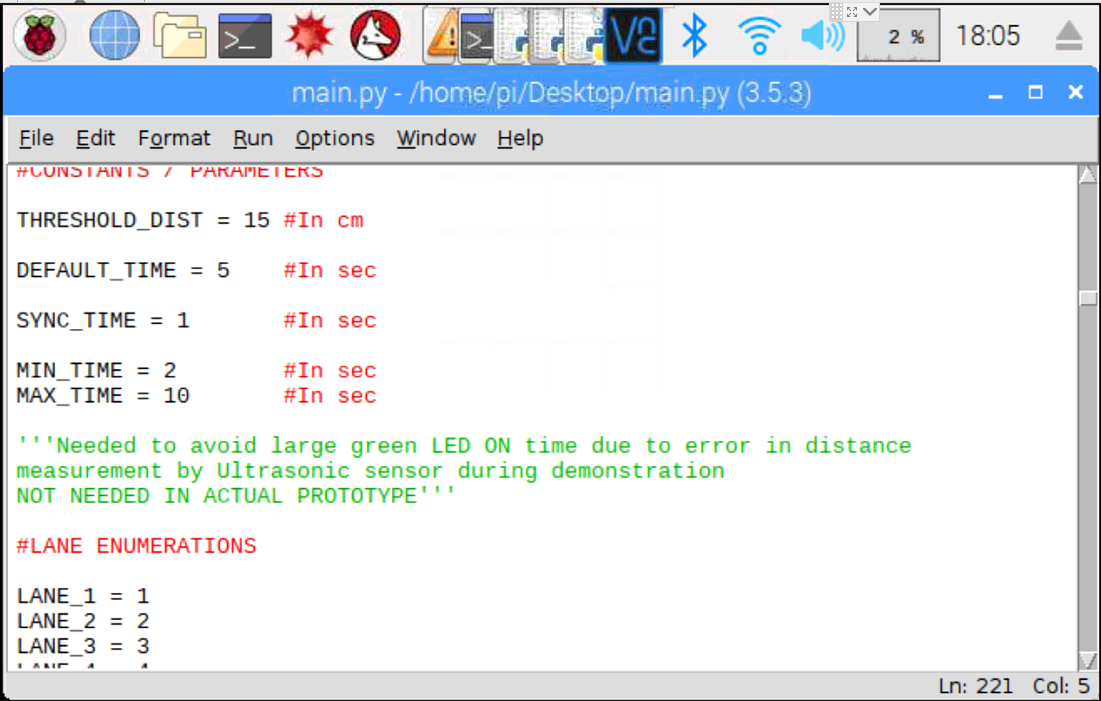
\includegraphics[width=5.5in]{./images/RunningCode.png}
\caption{IDLE IDE for Python}\label{RunningCode}
\end{figure}

Once the peripherals and sensors are connected to the RPI, the code is run with the help of python interpreter, which reads the traffic with the help of US sensor as explained and appropriately calculates the time for which the green signal is to be turned ON using the equations 4.1, 4.2 and 4.3.

\pagebreak

\subsection{Android App Control}

The system also reads the commands from the cloud parallely, to override any particular lane to be turned ON in case of emergencies. An android application is made, which controls the backend cloud data regarding which lane is to be overridden and so. It is powered by Ubidots, which is the most commonly used IOT platform that is used to send or receive data from micro-controllers to server and vice-versa. The android application is also equipped with login-based access to prevent unauthorized usage so as to prevent misuse of the application to control the signals unnecessarily. The lane override interface of the android application that is built is as shown in below figure,

\begin{figure}[h]\centering
        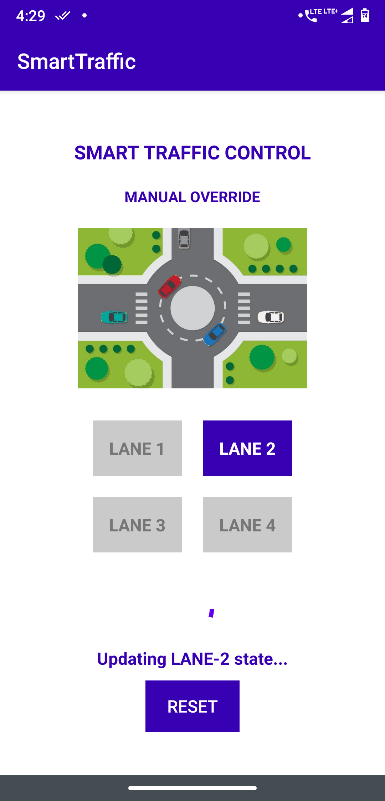
\includegraphics[width=2in]{./images/LaneOverride2.png}
        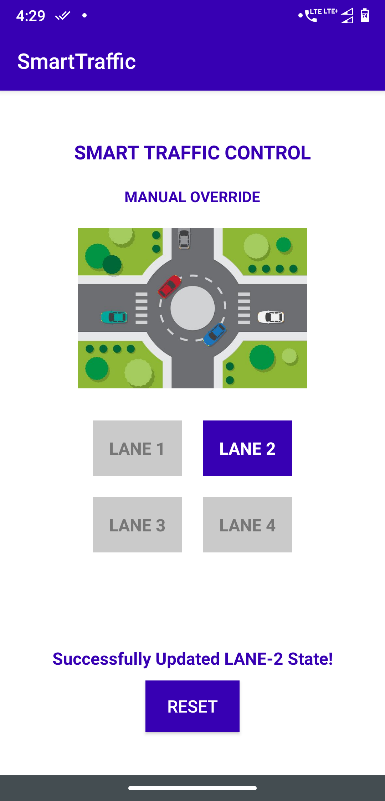
\includegraphics[width=2in]{./images/LaneOverride3.png}
	\caption{SmartTraffic Application - Lane Override}\label{LaneOverrideInterface}
\end{figure}


\pagebreak
